\section{Blockchain und Internet of Things}
Die Blockchain-Technologie bringt bereits einige Vorteile für Finanzsektor mit sich.
In der Kombination mit Internet of Things (IoT) lassen sich einige der bereits erörterten Einsatzgebiete
für breitere Anwendungsmöglichkeiten erweitern.
% IoT 
% kurz, dass ioT Daten sammeln können, die in der Blockchian gespeichert werden können und in Smart Contracts
% verarbeitet werden können

\subsection{Anwendungsmöglichkeiten/Synergien mit Internet of Things}

\subsubsection{Lieferkettenfinanzierung}
Integriert man IoT-Sensoren mit einer Blockchain-Struktur, können in der Lieferkette Zeit und Kosten bei
jeder Übergabe eingespart werden.
% Asset Tracking
Die IoT-Technologie schafft die Möglichkeit für Asset Tracking, um den Zustand von physischen Assets
kontinuierlich einsehen zu können. Durch das Anbringen von internetfähigen Sensoren an 
Liefercontainern kann so der Status des Transports vollumfänglich transparent gestaltet
werden und in Echtzeit abgefragt werden. 
Informationen die hierbei von Interesse sind, wären der aktuelle Standort der Lieferung und
die vorraussichtliche Ankunftszeit. Erweiternd dazu kann für empfindliche und 
verderbliche Waren die Temperatur, Luftfeuchtigkeit oder starke Erschütterungen auf dem 
Transportweg aufgezeichnet werden.
% Speichern und Smart Contract
Die Blockchain-Technologie bietet die Funktionalität, die erfassten Informationen in Blöcken
zu speichern. Damit fungiert die Blockchain wie ein Transportbericht der gesamten Lieferkette und 
sichert nebenbei die Integrität und Richtigkeit der Daten, sofern keine Sensorprobleme vorliegen. 
Zusätzlich kann bei der Zustellung der Lieferung ein Smart Contract die Zahlung automatisch ausführen.
So werden der Zeitaufwand und die Kosten für Qualitätsprüfungen reduziert und vor allem verderbliche 
Waren können schneller weiterverarbeitet werden.
Zudem können Finanzinstitute die Lieferkette
\cite[p.~169f]{chowdhary2025smart}


\subsubsection{Risiko-Management}
\label{sec:Risk_Management}
Der kontinuierliche Datenstrom von IoT-Sensoren kann zur Risikobewertung herangezogen, als auch zur 
Eingrenzung potentieller Schäden analysiert werden.
So können beispielsweise Versicherungsunternehmen die Daten aus einem Auto verwenden, sofern es eine 
Car2X-Kommunikation besitzt, um die Beiträge an das individuelle Fahrverhalten
anzupassen. 
Wenn die Sensoren oft einen riskanten Fahrstil melden, wie Geschwindigkeitsüberschreitungen oder 
nicht-einhalten von Mindestabständen, kann der Beitrag für die einzelne Person erhöht werden. Auf der 
Gegenseite kann sicheres Fahren mit niedrigeren Beiträgen belohnt werden. 
Dadurch ermutigt das Unternehmen zu einem vorsichtigeren Fahrstil, woraus weniger Unfälle resultieren 
können und daraus folgernd weniger Versicherungsansprüche gestellt werden.
\cite[p.~169f]{chowdhary2025smart}
Eine Anpassung des Beitrags kann ggf. erst nach längerem Beibehalten des Fahrstils automatisch mit einem 
Smart Contract vorgenommen werden.

Eine weitere Form Risiken einzugrenzen ist vorausschauendes Risiko-Management, welches die 
Betriebseffizienz steigern soll.
Eine mögliche Anwendung kann daraus bestehen, einen Leistungsbericht von Maschinen in einer Produktionskette
zu erstellen. IoT-Sensoren können hierfür einen kontinuierlichen Datenstrom als Basis für den Bericht liefern.
Aus dem Bericht können nachfolgen Leistungsschwankungen und -einbrüche erkannt werden und frühzeitig 
Gegenma\ss nahmen eingeleitet werden. Dadurch können Ausfälle der Produktionskette und damit einhergehende 
finanzielle Schäden minimiert werden.
\cite[p.~169]{chowdhary2025smart}

% Kreditrisiko in der Lieferkette \cite[p.~347ff]{Zhang2021Research}




\subsubsection{Smart Contracts und IoT}
% IoT Device Administration
Smart Contracts bieten die Möglichkeit die Verwaltung von IoT-Geräten zu automatisieren und zu dezentralisieren.
Mittels einer Blockchain kann ein System konstruiert werden, welches die Kommunikation zwischen IoT-Geräten
durch Blöcke realisiert. 
Vergleichsweise wird in zentralen Strukturen immer ein Intermediär benötigt, der beispielsweise ein 
Update-Request von einem Gerät A an ein Gerät B weiterleitet, welches dann das Update vornimmt.

Eine derartige Kommunikationsstruktur kann wie in \autoref{fig:SC-IoT_Update} dargestellt, umgesetzt werden.
Im ersten Schritt (1) schickt Device A einen Smart Contract an die Blockchain. Die Miner validieren diesen
und fügen den Contract in einem neuen Block hinzu (2 - 3). Dadurch besitzen alle Geräte, die Teil dieser 
Struktur sind, eine lokale Kopie des Smart Contract mit der Update-Funktion (4 - 5).
Nach der Verteilung der Daten ruft Gerät A die Update-Funktion in einer neuen Transaktion auf, welche 
wieder von den Minern in einem weiteren Block bestätigt wird (6 - 7). 
Der Smart Contract fügt bei der Ausführung einen dritten Block hinzu (8). Dieser beinhaltet ein Event,
welches den Update-Prozess auslöst.
Alle IoT-Geräte in diesem Netzwerk registrieren das Event und rufen die zugehörige Funktionalität auf, 
welches das Update durchführt (9). 
Anschlie\ss end schicken sie eine Bestätigung mit ihrem Status des Updates an das Netzwerk (10 - 11).

Auf diese Weise können Firmware-Updates und andere Software-Erweiterungen mit geringem Organisationsaufwand auf allen 
Geräten durchgeführt werden. 
Auch gerätespezifische Funktionalitäten eines IoT-Geräts können so von einem anderen Gerät aufgerufen werden.
Dieser Ablauf ist einfach skalierbar, da der Datenaustausch über Broadcasts stattfindet.  
Dadurch können beliebig viele IoT-Geräte dem Netzwerk hinzugefügt werden ohne den Kommunikationsaufwand 
proportional zu erhöhen. 
Zusätzlich sichern die Eigenschaften der Blockchain die Transparenz, Datenintegrität und Sicherheit der
Authentifizierung dieses Prozesses.
%Zusätzlich ist dieser Prozess durch die Eigenschaften der Blockchain transparent, 
\cite[p.~74f]{Choi2018DeviceControl}


% Wartungen von anderen Geräten (Smarte Geldautomaten)
Smart Contracts können auch zur Planung und Koordinierung von Wartungen oder zur Steigerung der 
Betriebseffizienz verwendet werden.
Leistungsberichte von IoT-Geräten (siehe Kapitel \ref{sec:Risk_Management}) können durch eine Erweiterung um 
Smart Contracts den Ansto\ss zum Wartungsprozess automatisieren.
% Wie im Kapitel \ref{sec:Risk_Management} erklärt, können Leistungsberichte von IoT-Geräten erstellt werden.
% Durch eine Erweiterung um Smart Contracts kann der Anstoß zum Wartungsprozess automatisiert werden. 
Bei einem festen Vertragspartner für Wartungen kann sogar der gesamte Prozess automatisiert 
werden. 
Der Contract kann bei der Ausführung eine Buchung zum nächstmöglichen Termin auslösen und bei Erfüllung 
der Wartung automatisch die Kosten begleichen.
\cite[p.~169ff]{chowdhary2025smart}

% Smart Contracts und IoT
\begin{figure}[!h]
    \begin{center}
        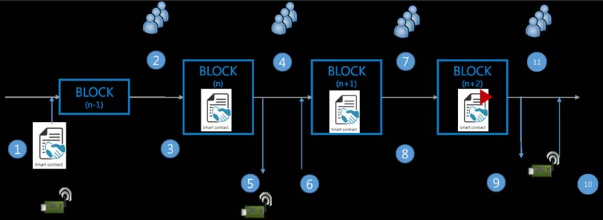
\includegraphics[height=5cm]{SC-IoT_Updating.png}
    \end{center}
    \quelle{\cite[p.~75]{Choi2018DeviceControl}}
    \caption{Kommunikation zwischen IoTs mithilfe von Smart Contracts}
    \label{fig:SC-IoT_Update}
\end{figure}



% \subsubsection{Asset Tokenization}


% \subsubsection{Analyse von Nutzerverhalten}

% Smart Wearables

% Fraud Detection durch ungewöhnliche Daten


\subsection{Herausforderungen und Risiken}

\subsubsection{Datensicherheit und rechtliche Risiken}
Die Eigenschaft von IoT-Geräten kontinuierlich Daten zu sammeln und zu teilen, ist für viele 
Anwendungsfälle erwünscht und oft der ma\ss gebliche Grund für deren Einsatz. 
Jedoch stellt ebendiese ein gro\ss es Risiko für den Datenschutz dar. Die Kombination mit der 
Blockchain-Technologie bietet bereits viel Sicherheit in Form von Datenintegrität und Schutz vor 
unauthentifizierter Datenmanipulation. Allerdings erfordert es zusätzliche regulatorische Bestimmungen, 
um vorallem Privatpersonen zu schützen.

Im privaten Kontext ist das mobile Banking der am häufigsten genutzte Service mit 
Blockchain- und IoT-Technologie.
Üblicher Datenverkehr beinhaltet hier Informationen über den Kontostand, die Transaktionshistorie, die
Kreditwürdigkeit und sogar biometrische Daten, die zur Authentifizierung verwendet werden.
Diese Daten gehören zu den sensibelsten und schützenswertesten, da ein Datenraub von diesen erhebliche 
Auswirkungen für die einzelne Person nach sich ziehen kann.
Mögliche Konsequenzen eines ungewollten Offenlegens können Finanzbetrug, unauthentifizierte Transaktionen 
und Identitätsdiebstahl sein. 
% Schutz
Um die Sicherheit bei der Nutzung solcher Dienste zu gewährleisten greifen einige Staaten auf Verordnungen
zurück. Mit diesen sind die Dienstleister dazu verpflichtet Richtlinien einzuhalten, welche die Daten über
die Blockchain-Eigenschaften hinaus schützen sollen.
Hierfür haben Europa die Datenschutz-Grundverordnung (DSGVO) im Jahr 2018 und die Vereingten Staaten
den California Consumer Privacy Act (CCPA) im Jahr 2020 einberufen.
In diesen ist sowohl die Selbstbestimmtheit über das Teilen der personenbezogenen Daten, als auch die 
Transparenz der Datennutzung spezifiziert.
Ein Nutzer muss demnach über die Art der gesammelten Daten und deren Verwendung in
Kenntnis gesetzt sein und der Nutzung explizit zustimmen.
%In diesen ist spezifiziert, dass ein Nutzer über die Art der gesammelten Daten und deren Verwendung in
%Kenntnis gesetzt sein muss und der Nutzung explizit zustimmt. 
%Die Transparenz für die Datennutzung kann
Eine etablierte Umsetzung hierfür sind Nutzungsbedingungen mit Zustimmungserklärungen.
Diese muss also eine Aufzählung aller erhobener Daten beinhalten und deren Verwendungszweck spezifizieren.
Der Nutzer muss vor der Erhebung jeglicher Daten allen Verwendungszwecken zustimmen.
In der Praxis empfiehlt es sich eine Zustimmung für jede optionale Dienstleistung separat zu erfragen.
% Hilfe
Dadurch bietet sich dem Nutzer eine individuelle Auswahl der Daten zu treffen, welche er bereit ist zu teilen.
Darüber hinaus muss der Nutzer stets die vollen Rechte über seine Daten besitzen.
Das beinhaltet das Recht alle personenbezogenen Daten einzusehen, welche gespeichert wurden und diese gegebenenfalls
ändern zu können. Au\ss erdem muss ihm die Möglichkeit auf das "Recht auf Vergessenwerden" geboten werden, 
wodurch alle gespeicherten Daten zu seiner Person gelöscht werden müssen.

Zusätzlich sind Finanzinstitute und IoT-Gerätehersteller dazu angehalten die Daten vor Hackerangriffen und 
Datenleaks zu schützen.
Die Unternehmen können eine hohe Cybersicherheit durch Verschlüsselung der Daten, regelmä\ss ige 
Sicherheits-Updates und sichere Authentifizierungsverfahren erreichen.
Eine Überwachung der Datenströme kann ebenfalls helfen Datenleaks schnell zu erkennen, falls atypische 
Bewegungen registriert werden.
\cite[p.~172]{chowdhary2025smart}
% Smart Contracts !!!


\subsubsection{Nachhaltiges Blockchain-Mining}
Nachhaltigkeit ist ein zunehmend ernstzunehmendes Thema, deren Umsetzung in vielen Bereichen eine 
Herausforderung darstellt. Um auch hier die Nachhaltigkeit in Betracht zu ziehen, wird hier die 
Funktionsweise der Blockchain auf ihre Ressourcennutzung untersucht. 
Die Blockchain-Technologie hat von Natur aus einen hohen Energieverbrauch um die Berechnungen für das 
Mining durchzuführen. Abhängig vom verwendeten Konsensalgorithmus existieren jedoch Unterschiede bei 
der Leistungsaufnahme. 
\cite[p.~2]{Athar2024BC_Sustainability}
Demnach bietet sich hier ein guter Ansatz, um Konsensalgorithmen hinsichtlich ihres Energieverbrauches
zu vergleichen.

Das Prinzip \glqq Proof-of-Work\grqq{} (PoW) benötigt von den hier betrachteten Algorithmen die meiste 
Energie um einen Rechnerknoten auszuwählen (vgl \autoref{fig:PoWPoS_Energy}). Dies kommt durch die vielen 
Berechnungsiterationen zustande, die benötigt werden um eine passende Nonce zu finden 
(siehe Kapitel \ref{sec:Erweiterung}).
\newline
Das Prinzip \glqq Proof-of-Stake\grqq{} (PoS) ist hingegen viel energieeffizienter 
(vgl \autoref{fig:PoWPoS_Energy}), da der Auswahlalgorithmus um einiges simpler ist.
Aus der \autoref{fig:PoWPoS_Energy} geht hervor, dass bei einem gemischten Konsesus-Modus bereits bei 
Modus 5 deutliche Energieeinsparungen im Vergleich zum reinen PoW im Modus 6 erkennbar sind. Demzufolge genügt ein Anteil von 20\% PoS im 
Gesamtgefüge, um die Leistungsaufnahme zu senken (vgl \autoref{fig:PoWPoS_Modes}).
Die Einfachheit des Algorithmus besteht darin, dass dieser seine Auswahl einzig von den Stakes abhängig
trifft. Die Stakes sind hierbei der Anteil an Kryptowährung, den ein Nutzer im Netzwerk besitzt.
Es wird der Nutzer gewählt, welcher die meisten Stakes oder mehr als ein Gro\ss teil der Nutzer besitzt.
Bei diesem Auswahlprinzip wird darauf vertraut, dass ein Nutzer mit vielen Stakes keinen Anreiz hat die
Daten zu manipulieren.
\cite[p.280]{Nair2021Energy}
\newline
Das letzte Prinzip \glqq Proof-of-Energy-Efficiency\grqq{} (PoEE) ist grundlegend auf eine hohe 
Energieeffizienz ausgerichtet. Die Auswahl eines Rechnerknotens wird anhand der nachgewiesenen Steigerung
der Energieeffizienz getroffen. 
Für den Nachweis werden analog zu Transaktionen auch die Energiesparma\ss nahmen auf der Blockchain 
gespeichert. Um weitere Anreize für die Reduktion des Energieverbrauchs zu schaffen, werden den 
Minern Prämien für Optimierungsma\ss nahmen angeboten.
So kann man einen Anteil der Kryptowährung erhalten, wenn beispielsweise die Spitzenlast im 
Energieverbrauch gesenkt wird oder erneuerbare Energien für das Mining genutzt werden. 
PoEE ist kompatibel mit anderen Konsens-Algorithmen und man kann diese verschachtelt strukturieren, um 
die Vorteile aus beiden zu nutzen.
Da PoW 
\cite[p.~2ff]{Athar2024BC_Sustainability}





\begin{figure}[!h]
    \begin{center}
        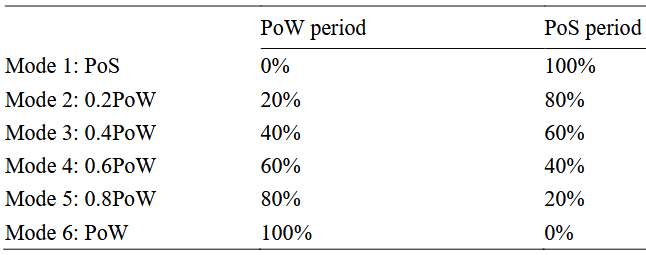
\includegraphics[height=5cm]{PoW-PoS_Modes.png}
    \end{center}
    \quelle{\cite[p.~3]{zhang2020PoWPoS}}
    \caption{Definition der Konsensus-Modi}
    \label{fig:PoWPoS_Modes}
\end{figure}

\begin{figure}[!h]
    \begin{center}
        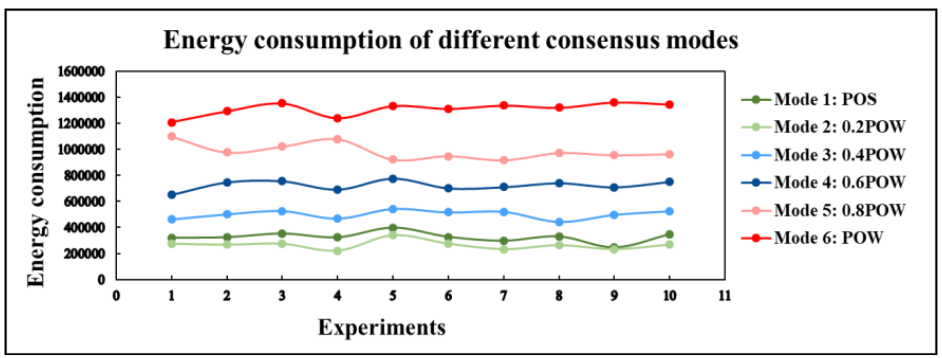
\includegraphics[height=5cm]{PoW-PoS_Energy.png}
    \end{center}
    \quelle{\cite[p.~4]{zhang2020PoWPoS}}
    \caption{Energieverbrauch der (gemischten) Konsensus-Modi}
    \label{fig:PoWPoS_Energy}
\end{figure}

%\cite[p.~2ff]{Athar2024BC_Sustainability}
%\cite[p.~279ff]{Nair2021Energy}
%\cite[text]{zhang2020PoWPoS}






% Chentara: Daten von Versicherungen und sonstige gespeicherte Daten sind öffentlich nur als Hashes einsehbar
% -> kein Rückschluss auf die eigentlichen Datenwerte möglich